\section{SECCIÓN 10. RECOPILACIÓN DE EVIDENCIAS, MANTENIMIENTO Y RETENCIÓN}
\textit{Identificar la documentación de SQA que se conservará, establecer los métodos e instalaciones que se utilizarán para reunir, salvaguardar y mantener esta documentación, y designar el período de retención.}

Las evidencias de pruebas y auditorías de calidad se almacenan en distintos medios según la herramienta empleada. En algunos casos, especialmente cuando la evidencia depende de ejecuciones previas o de entornos externos, es necesario volver a ejecutar la validación para poder consultar o recuperar la información, y únicamente se conserva la configuración o la salida generada por la herramienta.

\begin{table}[h]
    \centering
    \resizebox{\textwidth}{!}{%
        \begin{tabular}{|p{3.1cm}|p{3.2cm}|p{4.1cm}|p{2.8cm}|}
            \hline
            \textbf{Evidencia}              & \textbf{Formato de guardado}                              & \textbf{Ubicación}                                                                 & \textbf{Requiere ejecución} \\
            \hline
            Pruebas JUnit                   & Scripts en Spring Boot                                    & \texttt{src/test/}                                                                 & Sí                          \\
            \hline
            Pruebas frontend con Cypress    & Scripts                                                   & \texttt{frontend/cypress}                                                          & Sí, por consola o GUI       \\
            \hline
            Auditorías de dependencias      & Comando de consola / salida generada                      & Entorno de ejecución y reporte asociado                                            & Sí, para visualizarse       \\
            \hline
            Pruebas JMeter                  & CSV, XML o HTML                                           & \texttt{/jmeter/results}                                                           & No                          \\
            \hline
            OWASP-ZAP                       & Reporte HTML                                              & Ruta raíz del proyecto                                                             & No                          \\
            \hline
            Lighthouse                      & JSON y HTML                                               & \texttt{frontend/lighthouse-reports}                                               & No                          \\
            \hline
            SonarQube                       & Datos almacenados en contenedor de base de datos / Docker & Entorno Docker                                                                     & Sí, requiere activación     \\
            \hline
            Qlty.sh                         & Sin formato definido                                      & Nube                                                                               & No                          \\
            \hline
            Videos de ejecuciones de prueba & MP4                                                       & \url{https://drive.google.com/drive/u/1/folders/1UJUKMOLDKxPkp8ciLuoG23QkKwSRHRtN} & No                          \\
            \hline
        \end{tabular}%
    }
    \caption{Evidencias de calidad y su mecanismo de conservación.}
\end{table}

\subsection{Evidencias fotográficas}

Se adjuntan a continuación las evidencias fotográficas correspondientes a auditorías y reportes de calidad generados durante la ejecución de las actividades de SQA.

\begin{figure}[h]
    \centering
    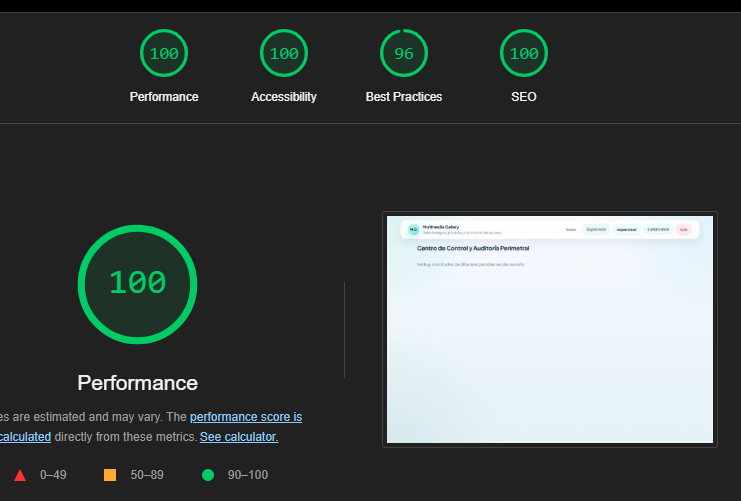
\includegraphics[width=0.8\textwidth]{images/evidencies/lighthouse.png}

    \caption{Reporte de Lighthouse}
\end{figure}

\begin{figure}
    \centering
    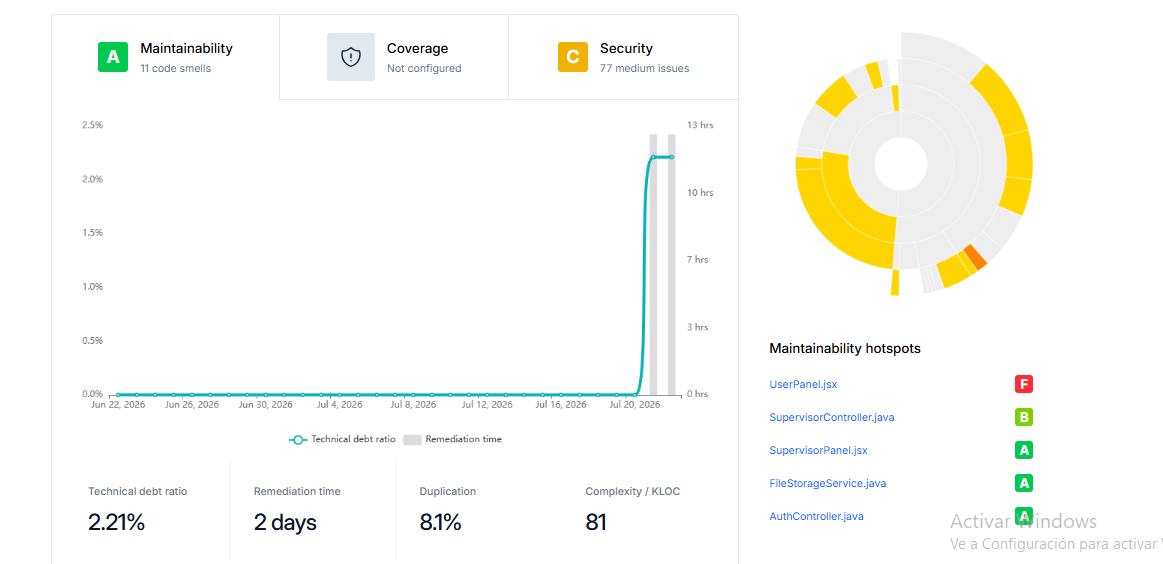
\includegraphics[width=0.8\textwidth]{images/evidencies/qlty_dashboard.png}
    \caption{Dashboard de Code Climate}
\end{figure}

\begin{figure}
    \centering
    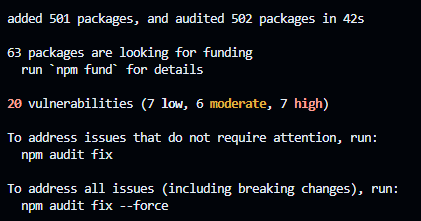
\includegraphics[width=0.8\textwidth]{images/evidencies/npm-audit.png}
    \caption{Evidencia de auditoría de dependencias}
\end{figure}